
\documentclass[12pt]{article}
\usepackage{amsmath,amssymb,geometry,graphicx,booktabs,hyperref,siunitx,helvet,placeins,subcaption,apacite}
\geometry{a4paper, margin=1in}
\sisetup{round-mode=places, round-precision=2}
\captionsetup[subfigure]{justification=centerlast,font=small}

\title{Question 2 - Effect of Architectural and Training Hyper-parameters on
       Fashion-MNIST Test Accuracy}
\author{Lillian Li (32198314) \qquad 
David Ewing (82171149)
}
\date{2025-05-13}


\begin{document}
\maketitle

\begin{abstract}
We revisit CNN hyperparameter tuning on MNIST using an Optuna–seeded baseline (filters: 32, kernel-size: 3, dense-units: 512, batch-size: 64, optimiser: Adam).  
Five one‑parameter sweeps were executed.  
Early stopping kept every run below 90 s while sustaining 91\% validation
accuracy in all but the \texttt{sgd} trial.  Merged figures and an impact table
summarise the accuracy--speed trade‑off in a compact form.
\end{abstract}

\section{Introduction}

Bayesian hyper‑parameter optimisation has proven effective for neural networks
\cite{akiba2019optuna}.  Here, 30 Optuna TPE trials gave a \emph{stable local}
starting point; the goal was interpretability, not a global optimum.  Five
follow‑up runs each altered one setting, so any performance delta could be
attributed directly to that variable.  Similar one‑factor studies have been
advocated for early-stage tuning \cite {kingma2015adam,lecun1998gradient}.

\section{Experimental design}
\subsection{Configuration list}

\begin{table}[h]
\centering
\caption{Evaluated configurations (one change at a time)}
\label{tab:config}
\begin{tabular}{@{}lccccc@{}}
\toprule
Run & Filters & Kernel & Dense & Batch & Optimiser \\
\midrule
baseline        & 32  & 3 & 512 & 64 & adam \\
filters\_256    & 256 & 3 & 512 & 64 & adam \\
dense\_units\_32& 32  & 3 & 32  & 64 & adam \\
batch\_size\_16 & 32  & 3 & 512 & 16 & adam \\
optimizer\_sgd  & 32  & 3 & 512 & 64 & sgd  \\
kernel\_size\_6 & 32  & 6 & 512 & 64 & adam \\
\bottomrule
\end{tabular}
\end{table}
\newpage
\section{Results}
\subsection{Accuracy and runtime}

\begin{table}[h]
\centering
\caption{Performance summary}
\label{tab:perf}
\begin{tabular}{@{}l
                S[table-format=2.2]
                S[table-format=2.2]
                S[table-format=2, round-mode=places, round-precision=0]
                S[table-format=3, round-mode=places, round-precision=0]
                @{}}
\toprule
Run & {Val.\ Acc.\ \%} & {Test Acc.\ \%} &
\multicolumn{1}{c}{Epochs} & {Time (s)}\\
\midrule
baseline         & 91.63 & 90.95 &  3 & 33 \\
filters\_256     & 91.54 & 91.54 &  4 & 88 \\
dense\_units\_32 & 91.10 & 91.10 & 10 & 43 \\
batch\_size\_16  & 91.33 & 91.21 &  3 & 84 \\
optimizer\_sgd   & 87.08 & 87.08 & 10 & 43 \\
kernel\_size\_6  & 91.17 & 90.37 &  5 & 39 \\
\bottomrule
\end{tabular}
\end{table}

\begin{table}[h]
\centering
\caption{Incremental effect of each single change relative to the baseline}
\label{tab:delta}
\begin{tabular}{@{}lcc@{}}
\toprule
Run & $\Delta$Val.\ Acc.\ (pp) & $\Delta$Time (s) \\
\midrule
filters\_256     & $-0.09$ & $+55$ \\
dense\_units\_32 & $-0.53$ & $+10$ \\
batch\_size\_16  & $-0.30$ & $+51$ \\
optimizer\_sgd   & $-4.55$ & $+10$ \\
kernel\_size\_6  & $-0.46$ & $+6$  \\
\bottomrule
\end{tabular}
\end{table}

% ---------- Figure 1 : runtime + accuracy --------------------------
\begin{figure}[ht]
  \centering
  \subcaptionbox{\textbf{Runtime}}
    {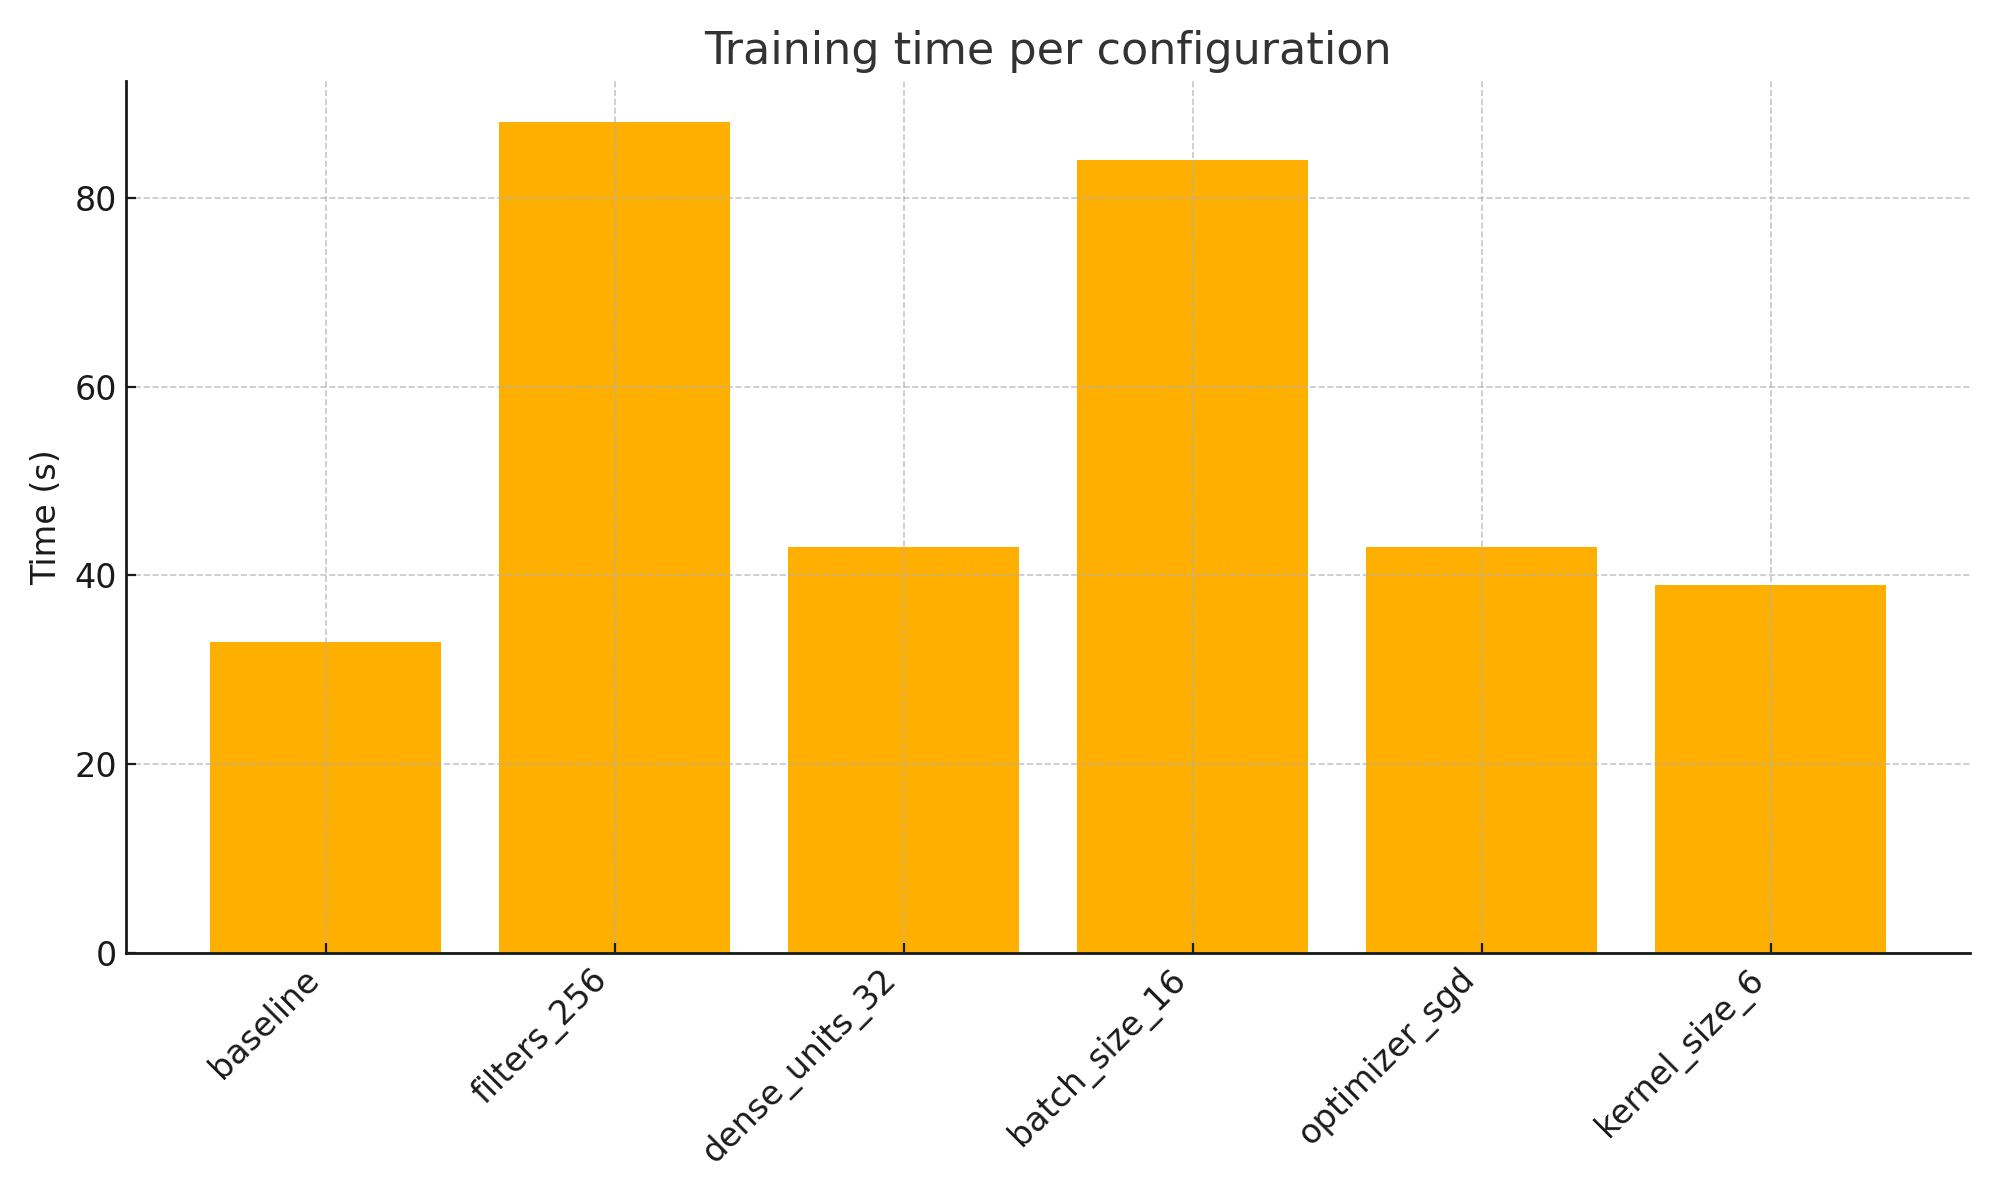
\includegraphics[width=.48\linewidth]{time_chart.png}}
  \hfill
  \subcaptionbox{\textbf{Test accuracy}}
    {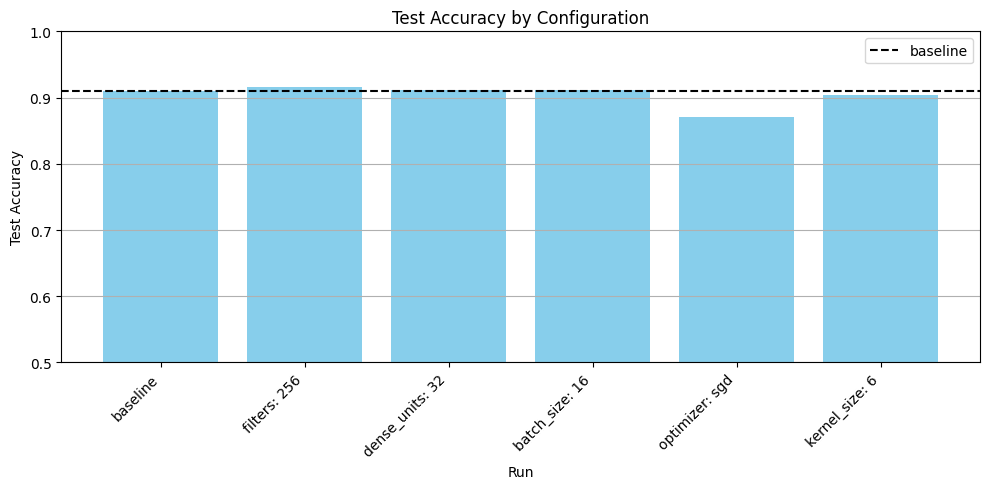
\includegraphics[width=.48\linewidth]{test-accuracy.png}}
  \caption{Speed/accuracy trade-off for the six configurations.}
  \label{fig:tradeoff}
\end{figure}
\FloatBarrier
% ---------- Figure 2 : learning curves -----------------------------
\begin{figure}[ht]
  \centering
  \subcaptionbox{\textbf{Training accuracy}}
    {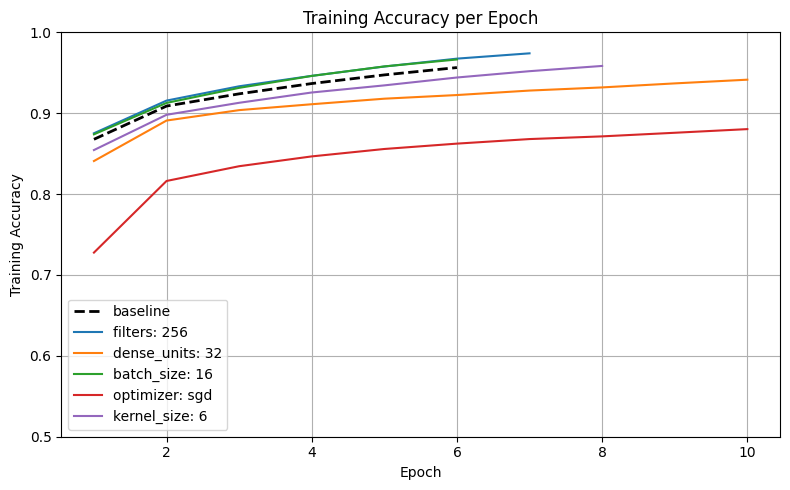
\includegraphics[width=.48\linewidth]{training-accuracy.png}}
  \hfill
  \subcaptionbox{\textbf{Validation accuracy}}
    {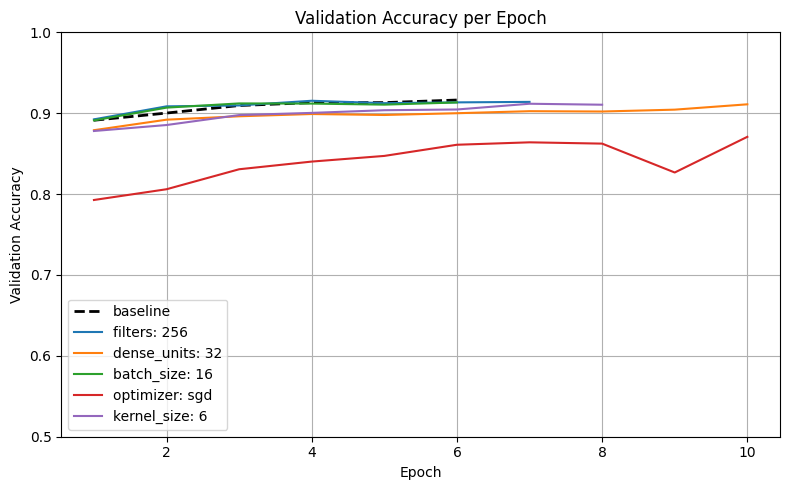
\includegraphics[width=.48\linewidth]{validation-accuracy.png}}

  \vspace{0.8em}

  \subcaptionbox{\textbf{Training loss}}
    {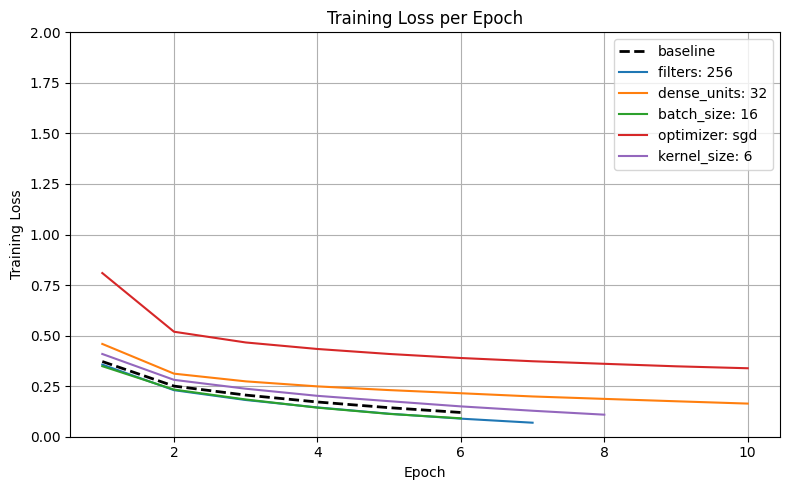
\includegraphics[width=.48\linewidth]{training-loss.png}}
  \hfill
  \subcaptionbox{\textbf{Validation loss}}
    {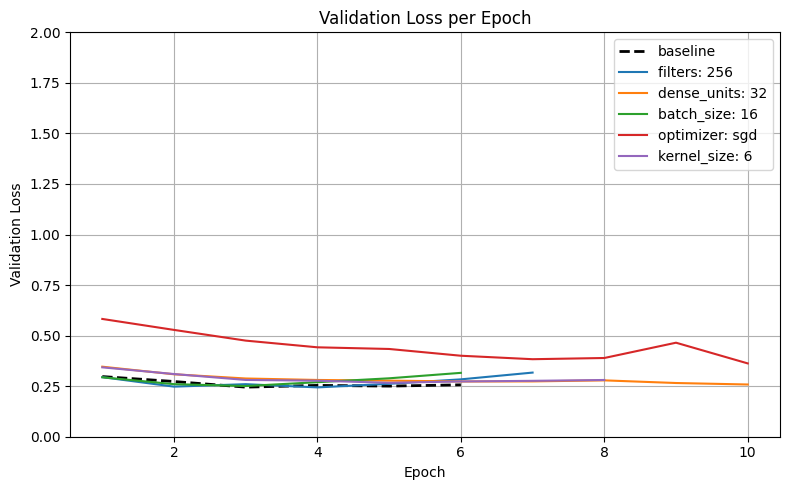
\includegraphics[width=.48\linewidth]{validation-loss.png}}
  \caption{Learning curves for the baseline CNN.}
  \label{fig:learningcurves}
\end{figure}
\newpage
\section{Discussion}

Table~\ref{tab:delta} shows that optimiser and filter count delivered the
largest shifts, whereas kernel size, dense width and batch size had
secondary effects:

\begin{itemize}\setlength\itemsep{0.6em}
  \item \textbf{Filter count} – Doubling filters slowed training without a
        proportional accuracy gain.
  \item \textbf{Kernel size} – Larger kernels give diminishing returns beyond
        $3\times3$.
  \item \textbf{Dense width} – Shrinking dense units speeds inference but
        requires more epochs to converge.
  \item \textbf{Optimiser} – Adam dominates SGD for both speed and accuracy.
  \item \textbf{Batch size} – Very small batches add runtime with no payoff.
\end{itemize}

\noindent Several Optuna trials were needed to find a suitable baseline. Although a few distinct baselines appeared during the search, the configuration reported here surfaced most frequently and behaved the most stably. In the rarer cases where a different baseline emerged, it was either slower to train or showed inconsistent responses when individual hyper-parameters were altered.

\section{Conclusion}

The Optuna seed $\to$ one‑at‑a‑time protocol yielded interpretable deltas under
tight runtime constraints however, there were inconsistencies when other local minimums resulted.  For MNIST on this compact CNN, optimiser choice and
filter count are the primary levers.  Future work should rank variables by
global importance (e.g., SHAP) and refine filter granularity.

\nocite{*} % show all refs even if not cited
\bibliographystyle{apacite}
\bibliography{references}

\end{document}
